\documentclass{article}
\usepackage[a4paper, top=3cm, left=3cm, bottom=3cm, right=3cm]{geometry}
\usepackage[T1]{fontenc} 
\usepackage[utf8]{inputenc} 
\usepackage[italian]{babel} 
\usepackage{lipsum} 
\usepackage{url} 
\usepackage{lmodern}
\usepackage{graphicx}
\usepackage{psfrag}
\usepackage{amsfonts}
\usepackage{amsthm}
\usepackage{amsmath}
\usepackage{amssymb}
\usepackage{mathrsfs}
\usepackage{tikz-cd}
\usepackage{mathtools}
\usepackage{tikz} 
\usepackage{caption}
\captionsetup{labelformat=empty,textfont=sl}
\usetikzlibrary{decorations.markings}
\usepackage{enumitem}
\usepackage[hidelinks]{hyperref}
\usepackage[numbered,framed]{matlab-prettifier}

\lstset{
  style              = Matlab-editor,
  basicstyle         = \mlttfamily,
  escapechar         = ",
  mlshowsectionrules = true,
}

\title{\textbf{Laboratorio Sperimentale di Matematica Computazionale / / Mimosa con rumore (F3)}}
\author{Dario Rancati - 539365} 


\begin{document}

\maketitle

\noindent
Lo scopo della sperimentazione corrente è quella di applicare il metodo di filtraggio immagini mediante FFT studiato a lezione con 
i filtri $f_{j}$ seguenti:

$$f_{j}= 1 - \cos{\left( \frac{3\pi}{2}+\frac{2j\pi}{n} \right)} \; \; j = 0, \ldots \frac{n}{2}$$

\noindent

Che, come si vede dal loro grafico riportato nelle slide, sembrano die filtri "passa medio", che filtrano sia frequenze alte che basse. L'immagine a cui vogliamo applicare il filtraggio è la seguente:

\begin{figure}[!h]
\centering
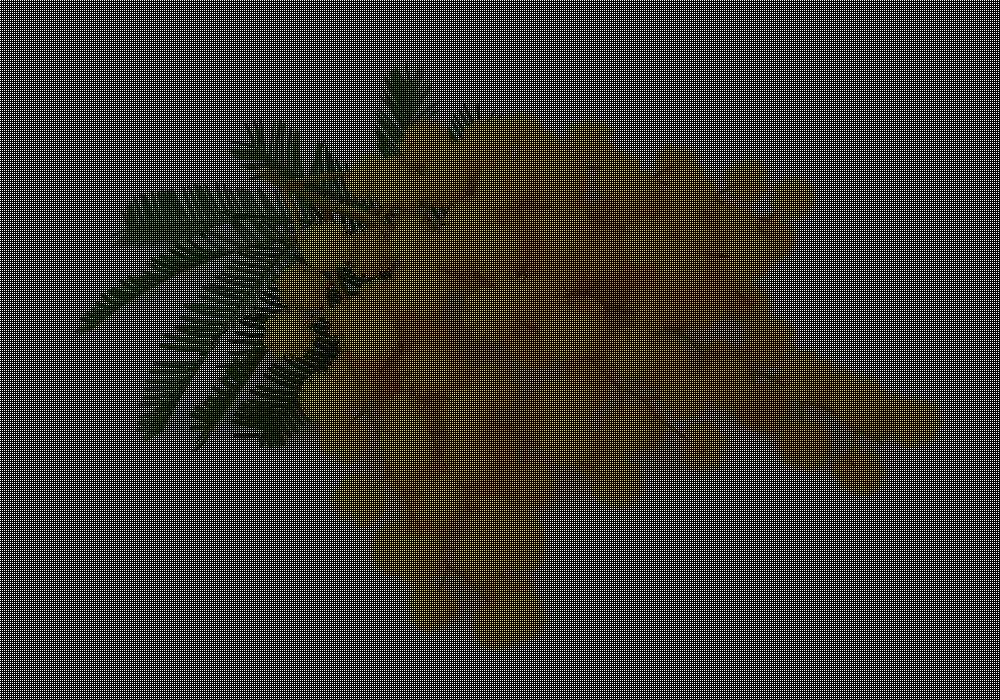
\includegraphics[width=\textwidth]{mimosar.jpg}
\end{figure}

\noindent
La function che effettua il filtraggio in funzione dei generici filtri f1 e f2 è la seguente: l'abbiamo ottenuta modificando leggermente la \texttt{filtra} delle slides, facendo sì che il filtraggio avvenisse per ciascuna delle tre componenti dello standard rgb:

\begin{lstlisting}
function W = filtra_rgb(V, f1, f2)
  % calcolo fft di righe e colonne
  V = double(V); 
  u1 = fft2(V(:,:,1));
  u2 = fft2(V(:,:,2));
  u3 = fft2(V(:,:,3));
  U(:,:,1)=u1; 
  U(:,:,2)=u2; 
  U(:,:,3)=u3;
  %qui abbiamo applicato la fft a ciascuna delle tre coponenti dello
  %standard rgb
  % filtro e antitrasformo sempre secondo lo standard rgb
  Z1=diag(f1)*U(:,:,1)*diag(f2);
  Z2=diag(f1)*U(:,:,2)*diag(f2);
  Z3=diag(f1)*U(:,:,3)*diag(f2);
  Z(:,:,1)=Z1; Z(:,:,2)=Z2; Z(:,:,3)=Z3;
  w1 = ifft2(Z(:,:,1));
  w2 = ifft2(Z(:,:,2));
  w3 = ifft2(Z(:,:,3));
  W(:,:,1)=w1;
  W(:,:,2)=w2; 
  W(:,:,3)=w3;
  % ripulisco
  W = real(W); % tolgo eventuale roundoff immaginario
  W = uint8(W); % trasformo variabile double in intera
  % riportando i valori tra 0 e 255
\end{lstlisting}

\noindent
Il seguente è lo script che esegue il filtraggio dopo aver calcolato i filtri f1 ed f2. Notiamo che le proprietà di parità del coseno ci consentono una scrittura molto compatta dei vettori, che non richiede nemmeno di separare i casi per parità/disparità. Abbiamo aumentato la luminosità sommando una matrice di tutti 1, in quanto il metodo usato nelle slides schiariva decisamente troppo:

\begin{lstlisting}
X=imread('mimosar.jpg');
[n,m,l]=size(X);
j = [0:n-1];
%costruiamo i filtri f1 e f2
f1= 1-cos(3*pi/2 + pi*j/n);
j = [0:m-1];
f2= 1-cos(3*pi/2 + pi*j/m);

Y = filtra_rgb(X,f1,f2);
%schiariamo
Y = Y+100*ones;
Y = uint8(Y);
imshow(Y);
\end{lstlisting}

\noindent
Infine, questa è l'immagine filtrata:

\begin{figure}[!h]
\centering
\includegraphics[width=\textwidth]{mimosaf.jpg}
\end{figure}

\end{document}